\chapter{Designing and Building the System} \label{development}

\begin{quote}
\emph{This Chapter describes the requirements for a system built upon
  Blockchain technology. The requirements where chosen in order to create a
  system that is interesting to an organization while still respecting the
  patients data access rights. Ethereum and Hyperledger Fabric advantages and
disadvantages were weighted for this use case. Finally, insight into the design
and implementation of the system is given.} \end{quote}

The goal of this dissertation is to create a solution to manage the identity of
patients in an Healthcare organization by conceptualizing, implementing and
evaluating a Blockchain based system that fulfills this role. In order to
fulfill this goal, the development part of the work described in this
dissertation was primarily divided into four steps with each step building upon
the previous ones. The development workflow spans the conceptualization and its
associated challenges and ends in the implementation of said system.

\section{First Step - Defining Requirements and Choosing a Platform}
\label{choosingHyperledger}

After investigating the various Blockchain platforms some criteria was needed
to serve as reference. As such, the first step consisted in defining a set of
key points that the built system had to fulfill. Defining the requirements
proved helpful to choose the most appropriate platform for the objectives as
explained later.

\subsection{Requirement Definition} 
The requirements for this work were deemed to be as follows:

\renewcommand{\labelenumi}{\Roman{enumi}.}
\begin{enumerate}
  \item The system must allow a patient to opt into the network and register as
    a participant.
  \item The system must allow a patient to record his medical data under the
    approval of an administrator.
  \item The system must keep data confidential, transparent and have
    high availability.
  \item The system must provide the patient with the ability to share his data
    with another entity, for example sharing information with a doctor.
  \item The system must allow the deletion of a patient's data in some manner,
    if he wishes to do so, in order to comply with European privacy laws,
    discussed in Section~\ref{blockchainHealthcare}.
\end{enumerate}

These requirements were chosen in order to create a system that is interesting
to an organization while still respecting the patients data and their access
right to it. 

After defining the requirements it was nececessary to choose the Blockchain
platform that best fulfills these requirements.

\subsection{Choosing a Platform}\label{choosePlatform}

Even tough Blockchain platforms normally originate from the realization that
full centralization has major drawbacks, they often have different goals. These
translate into architectural differences and different development focuses.
These range from open networks, such as Ethereum which anyone can join and use,
to permissioned distributed ledgers, which can be run publicly or privately but
are only open to access and participation through a membership service, such as
Hyperledger Fabric and Hyperledger Indy.

Ethereum has a growing learning ecosystem and community. It is easy to start
interacting with the network as anyone is able to simply download a client and
connect to it. Thanks to the Solidity (see Section~\ref{ethereumPlatform})
smart contract language being targeted for the specific purpose of authoring
smart contracts it only allows for a deterministic program to be written
avoiding potential conflicts in the execution of these, for example, in the
production network. Since Solidity is a Domain Specific Language it is platform
easy to develop for since it provides a well thought out and well organized
documentation with an easy to use library of operations.

Ethereum is being used in a great deal of projects around the world proving its
stability and suitability in a wide variety of use cases. On the other hand,
handling patients medical data is a great responsibility due to the private and
personal nature of this data. Also hospitals and Healthcare clinics must obey
the regulatory laws regarding privacy and usage of this data.

It is also worth noting that while Ethereum can handle private data exchange by
building upon it, as shown by Barclay in his dissertation, it was not designed
with this intent in mind, therefore these middle ground solutions can prove to
be unwise to use at scale given Ethereum's and the whole Blockchain's ecosystem
past problems with scalability.  

Fabric, like Ethereum, was built with the intention of being a general purpose
use Blockchain. It provides developers with the tools needed to build any
system they can imagine. The latter is clearly focused on making organizations
feel more at ease by being auditable. It is auditable because it offers an
identity service by using a membership service provider and a private
certificate authority that emits certificates specific for the Fabric network.
These concerns allow this platform to avoid the same fate Internet of Things
devices have had in the Healthcare field~\cite{Tana2017} where the lack of
security regulations and ambiguity in how data was being collected by these
devices has limited their usage and prevented the widespread usage of these
devices in the Healthcare field.

Fabric also has a good amount of development tools that are now maturing and a
good learning environment with ample documentation about every aspect important
for a developer looking to get started into it. Fabric is being backed by the
Linux Foundation and IBM, lending credibility to the project and ensuring that
this platform is supported and developed into the foreseeable future, as it is
being governed by a diverse technical steering committee and by a diverse set
of maintainers from multiple organizations. In regards to performance, the
focus in this area is clear, as the Hyperledger community has appointed a
Performance and Scale working group to improve performance as well being tasked
to implement benchmarking framework for Hyperledger projects called Hyperledger
Caliper~\cite{performanceScale2017}.

Regarding Fabric's features, it lends itself very well to fulfill the project
requirements. Fabric's channels and private data segregation at peer level make
a clear statement that privacy is important in this platform, which is in line
with the requirements that were laid out for the work described in this
dissertation. It is also worth noting that many upcoming Blockchain based
projects in the Healthcare field are using permissioned networks due to these
same concerns regarding the patients privacy while retaining the key benefits
of Blockchain such as immutability and decentralization. The fact that Fabric
has no associated currency also means there is no required mining incentives to
maintain the network, even tough it does require some additional infrastructure
to set up the network, leading to a higher initial investment in a solution
based on this platform.

Both are very interesting platforms, but ultimately it was decided to use
Hyperledger Fabric as the platform on which to build upon. This decision was
taken in part because Fabric was purpose built for a very regulated environment
and is focused on privacy and scalability which are required in the Healthcare
field. Also, this technology is relatively recent and there is still a great
lack of knowledge available to the general public, making it a more interesting
choice from an theoretical standpoint.

\section{Hyperledger Fabric Components and Administration}

After selecting Hyperledger Fabric as the work platform, it became necessary to
understand in further detail what are the main components that form a network
and the tools available to manage these components. This Section discusses the
main components of a Fabric network and the tools required to create and
maintain a Fabric network. These components often interact with one another and
provide the technical infrastructure that comprises this technology.

\subsection{Hyperledger Fabric Components}

An Hyperledger Fabric (HLF) network is defined as the technical infrastructure
that provides ledger and smart contract services to applications. Smart
contracts are used to generate transactions and interact with the ledger. The
network is comprised of several components, which are described in the
following paragraph.

The ledger is a central component of a HLF network. The ledger is composed by a
world state and a Blockchain as seen of Figure~\ref{fig:ledgerFabric}. The
world state is a database that holds the current values of ledger states.
States are, by default, expressed as key-value pairs. The world state is useful
because it makes it easy for a smart contract to get the current value of these
states, instead of having to traverse the entire transaction log. The
Blockchain holds the transaction logs that record the history of changes that
have resulted in the current world state.

Finally, transactions are collected and recorded in an immutable sequence of
blocks, in which each block contains a set of ordered transactions by the
orderer service.

\begin{figure}[ht] 
	\centering
	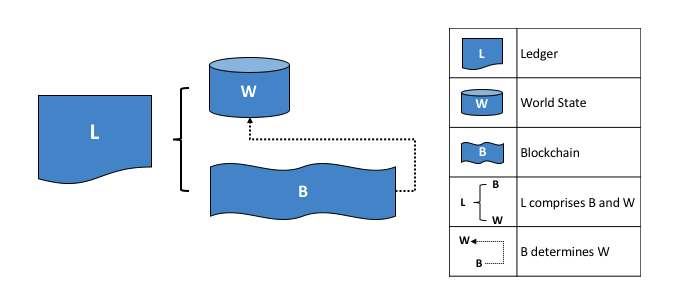
\includegraphics[width=1\linewidth]{imgs/ledgerFabric.png}
  \caption{\label{fig:ledgerFabric}Fabric's Ledger Overview (Source:
  \href{https://hyperledger-fabric.readthedocs.io/en/release-1.2/ledger/ledger.html}{HLF
  Fabric Documentation})}
\end{figure}

Another component is the set of peers participating in the network. A peer is a
node that hosts a copy of the multiple ledgers and smart contracts. There is
one logical ledger in a Hyperledger Fabric network, even tough, in reality the
network maintains multiple copies of a ledger that are synchronized through
consensus. HLF opts to allow multiple ledgers in a network to achieve different
goals of a greater purpose. This allows the creation of channels of information
between trusted parties, for example, a channel of secure and private
information between the clinical staff of an hospital and a patient as
discussed on Chapter~\ref{background}, in which every channel has a ledger.

Through a peer connection, applications execute chaincode that queries or
updates a ledger. Peers have at least one of the three different roles assigned
to them, as seen on Section~\ref{distributedLedgerPlatform}. Applications
always connect to peers when they need to access ledgers and smart contracts.
Every peer in the network is assigned a digital certificate by an administrator
from its owning organization. The mapping of a peer's identity in an
organization is provided through the membership service provider. 

Peers, applications, end users (clients), administrators, channels and
organizations must have an identity provided by the Membership Service Provider
(see Section~\ref{distributedLedgerPlatform}) in order to be able to interact
with the network. Each of these actors has a digital identity encapsulated in
an X.509 digital certificate standard which must be unique to every entity.
These determine the exact permissions these have over resources and access to
information in the network. The MSP issues these certificates through the
built-in Certificate Authority (CA) component, the Fabric CA. The Fabric CA is
a private root CA provider that consists in a CA server and a CA client. The
MSP also supports Certificate Revocation Lists as seen in
Figure~\ref{fig:membershipFabric}.

\begin{figure}[ht] 
  \centering
  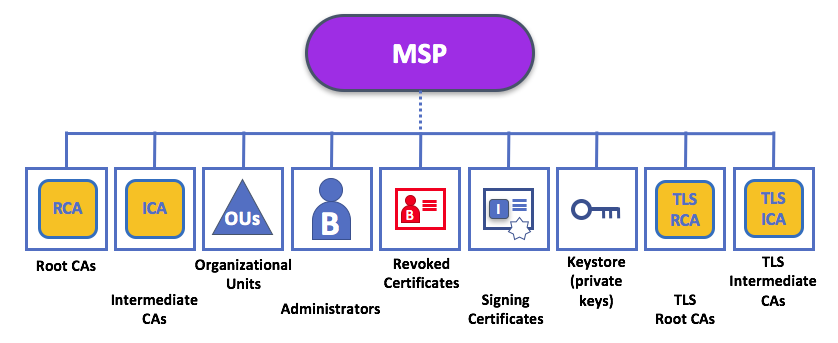
\includegraphics[width=0.9\linewidth]{imgs/membershipFabric.png}
  \caption{\label{fig:membershipFabric}Fabric's Membership Service Provider
  Components Overview (Source:
  \href{https://hyperledger-fabric.readthedocs.io/en/release-1.2/ledger/ledger.html}{HLF
  Fabric Documentation})}
\end{figure}

\subsection{Administrating a HLF Networks}

As discussed, a HLF network must have an administrator. HLF provides the
\textit{cryptogen}, \textit{configtxgen}, \textit{configtxlator} and
\textit{peer} tools that are used to configure the network to suit different
needs and use cases.

The \textit{cryptogen} tool generates cryptographic data consuming the file
\textit{crypto-config.yaml}.

The \textit{configtxgen} tool generates the genesis block for the orderer
services (see Section~\ref{distributedLedgerPlatform}) and the initial
transactions.  This tool consumes the file \textit{configtx.yaml} that defines
configuration parameters for channels, the genesis block and the orderer
service.

The \textit{configtxlator} tool is also used to generate channel
configurations.  Finally the \textit{peer} tool is used to manage the
participating peers in the HLF network.

These tools are used to create and maintain the topology of the network and are
invoked when a change to the network is made, for example, when permissions to
certain records are changed or a new user is enrolled in the network and are
very much intertwined with the Fabric Certificate Authority (CA) discussed in
subsection .

\section{Building the System}

After considering the project goals of investigating the suitability of a
Blockchain based system to manage patients identity data in Healthcare, the
third step was to build a prototype of a system that would provide a simulation
of the production network, albeit on a smaller scale. The insights gained from
developing a simple working system would enable benefits and risks of the
approach to be identified, and opportunities for further research to be laid
out.

In order to build a solution, the research done before hand was taken into
account and allowed a global overview of how architecturally a system could be
built with the components available. After some consideration some approaches
were reached, which are hereby presented in the following sections.

\subsection{Conceptualization and Design}

After an analysis of the defined requirements and the platform chosen, it was
determined that the information that defines the patient's identity is a key
requirement to build a system that recognizes patients across the Healthcare
environment, as discussed in Chapter~\ref{background}. An asset could be
created through chaincode that represents the concept of the patient's identity
in this network. This asset is stored in a Fabric network as a key-value pair.
The key for this kind of asset could be a string. This string could be composed
by the string 'Patient\_', followed by a patient identification number assigned
when the data is entered into the Blockchain. Since optimization is not a key
concern to build a simple prototype in the context of the work described in
this dissertation, the patient's identification number was defined to simply be
the order of the data entry starting at number one. This ensures that the key
is unique and it is easily computable. In short, it was decided that the key is
formed by the string 'Patient\_' followed by the mentioned patient
identification number. This key is used to query and access the patients data.

To aid in interoperability with other systems, the Fast Healthcare
Interoperability Resources (FHIR) standard by the Health Level 7 organization
could be used as basis for the fields in the structure used to represent the
patient's identity in the Healthcare domain.  Each field of the patient's
identity structure, defined in a smart contract, would be linked to a field of
the \href{http://www.hl7.org/fhir/patient.html}{patient structure as presented
in the FHIR standard}.

The most simple case of an interaction in an Healthcare service is the
interaction between a patient and a doctor. In HLF, this situation translates
to two organizations and two peers. Each peer belongs to an organization, one
organization represents the patients while the other represents the hospital
where the doctor works. 

To establish a communication between the two participating peers, a channel is
created between the peers, ensuring information exchanged between the two is
private and does not exist on the rest of the network.  If a third organization
with another peer representing another health clinic joined the network, then
another channel could be created between the patient's organization and this
new organization. If the patient inserts his data in the channel then the
clinic would be able to view it everytime they wished. 

Starting in version 1.1 of Fabric the MSP allows Attribute Based Access Control
meaning the access to the data can depend on the value of certain attributes of
the certificate. Also it is possible to encrypt data and insert it into the
channel and then require a key to decrypt the data. In this case the patient
could give a key to the doctor to be able to access only his data. In the
current version of Fabric, version 1.2, private data collections were
introduced~\cite{hyperledgerRoadmap2018}, meaning that some data can be marked
as private on a channel while other data can be public.

\subsection{Implementation}

Applications for Hyperledger Fabric can be developed in any language as long as
there is a Software Development Kit (SDK) supporting the chosen language. At
the time of writing this document, the Node.js SDK and the Java SDK are
available with additional language support being worked
on~\cite{hyperledgerRoadmap2018}.

To create an interactive system that can manage the patients identity in an
Healthcare environment, an application was built using Node.js that the user
interacts with. Node.js is a JavaScript runtime built on Google Chrome's V8
JavaScript engine. Node.js has an event-driven architecture focused on
asynchronous input/output which optimizes the throughput and scalability of web
applications with many input/output operations. In short, Node.js allows
JavaScript to be run in the Node.js environment allowing for the creation of a
command line interface tool, for example.

In regards to developing smart contracts or chaincode, Go was the first
programming language to get support and since then additional languages were
added to the list of officially supported languages. At the time of writing
this document, the Go language SDK and Node.js SDK are available and the Java
SDK was also recently released. 

After some research, the Node.js SDK for developing chaincode had similar
features in comparison with the Go SDK, in regards to API and features.
However, documentation was more sparse and harder to find for the Node.js SDK. 

On the other hand JavaScript was more approachable in contrast to Go, in order
to implement the system due to the author's familiarity with the Node.js
environment. Another important consideration is that, the application and the
smart contract could both be built in this language which was considered an
advantage as it simplifies dependency management. 

Ultimately, this application interfaces with chaincode through the Hyperledger
Node.js Fabric Software Development Kit. The chaincode was developed using the
Hyperledger Fabric Shim for Node.js.

To avoid the need for multiple machines being created in order to form the
network, a Docker Compose file was used that defines, and orchestrates the main
components of the network through the Docker Engine. Docker is a platform that
allows containerization~\footnote{Containerization, refers to an operating
system feature in which the kernel allows the existence of multiple isolated
user-space instances without launching an entire virtual machine for each
application. These instances, called containers, share the host operating
system and hold only the application related binaries and libraries, thus being
more lightweight and faster than virtual machines.}. The Docker Engine is an
open source containerization technology offering a workflow for building and
containerizing applications. A Docker Compose file specifies the topology of
the service stack and allows orchestration of the services therein defined.
With this in mind, each component of the network consists in one or more
containers, with one container defined to be used as a command line interface
to interact with the network using the peer tool, if needed for administrative
purposes. Docker was used as the containerization technology because it is
officially supported by Hyperledger and is currently the most popular
containerization tool as of
2018~\cite{dockerAdoption2018,containerAdoption2018}.

To build the desired network configuration for the prototype, the configuration
file for the \textit{cryptogen} tool was modified to allow the network to have
two organizations, each of them with a peer associated. The configuration file
for the configtxgen tool was also edited to allow a channel of information
between the two organizations to be created. Each peer would serve as the
anchor peer~\footnote{Used to initiate communication between peers from
different organizations. The anchor peer serves as the entry point for another
organization’s peer on the same channel to communicate with each of the peers
in the anchor peer’s organization.} in each of the organizations.

An application was also built that allows for user enrollment to create a new
identity in the network. The application is run by a user and uses the
available SDK to call upon the operations that the smart contract makes
available. When a new user of the application enters the network, a function in
the smart contract initializes the creation of the patient's data and writes
the patient's Healthcare information to the ledger as a new asset, and also
manages the ledger state through transactions as well as the world state. The
overview of the architecture for this system is represented on Figure
\ref{fig:appOverview}. Due to the security mechanisms these transactions are
signed and endorsed by the administrator of the network and verified by the CA
servers.

\begin{figure}[ht] \centering
  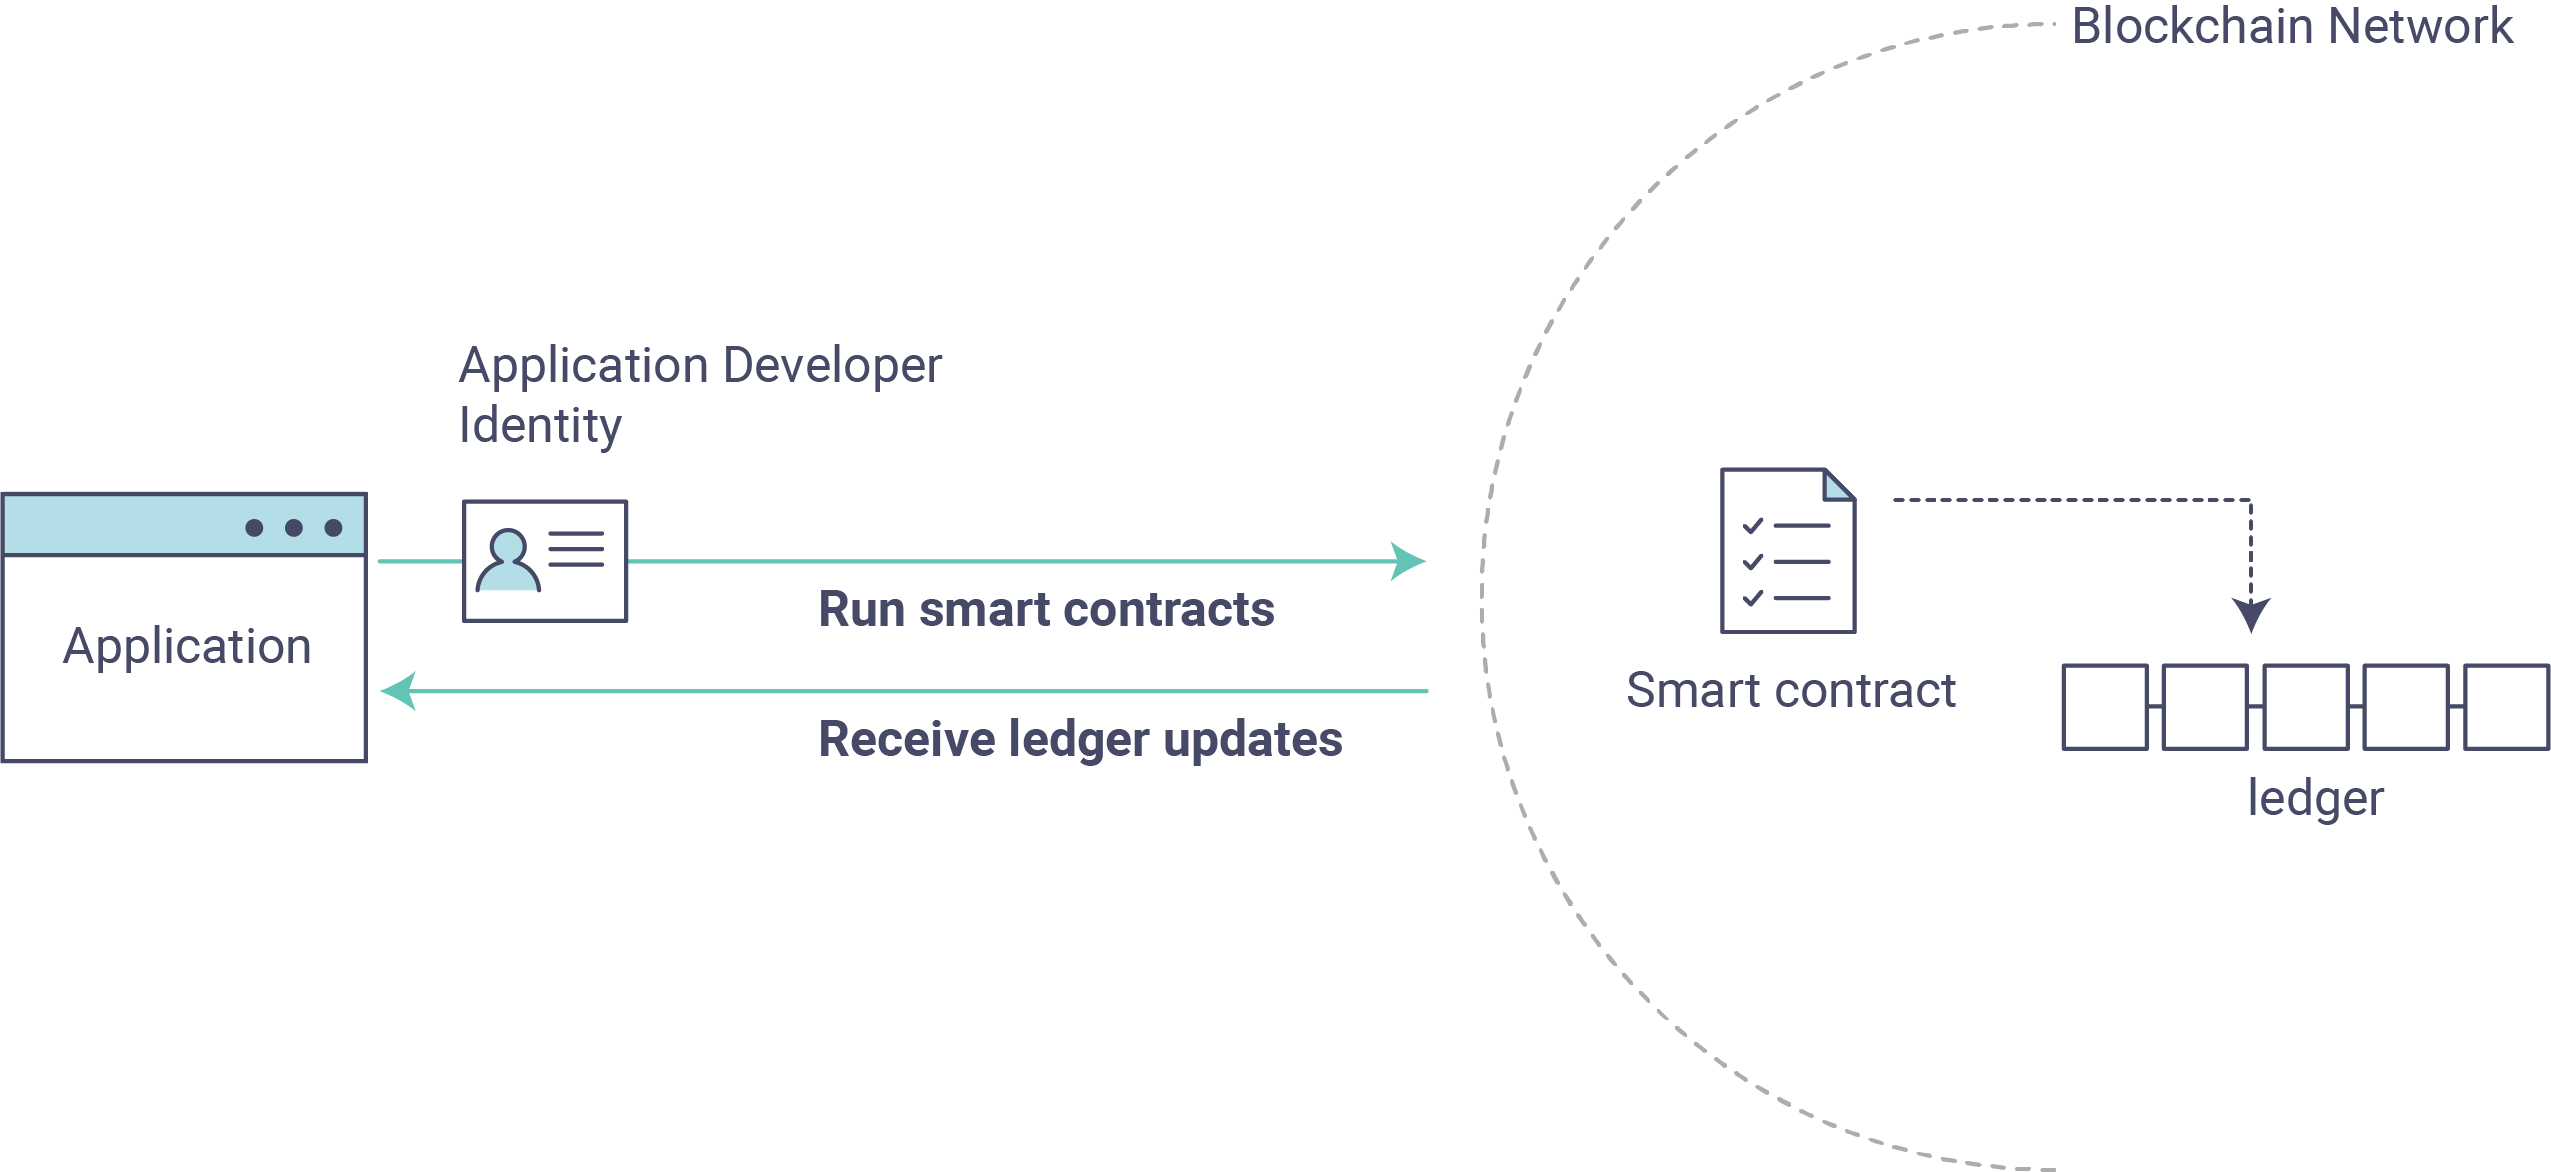
\includegraphics[width=0.83\linewidth]{imgs/hyperledgerAppOverview.png}
  \caption{\label{fig:appOverview}An Overview of the System Architecture
  (Source:
  \href{http://hyperledger-fabric.readthedocs.io/en/latest/write_first_app.html}{HLF
  Fabric Documentation})} 
\end{figure}

The assets loaded contain the necessary fields to identify a patient in an
Healthcare context, such as its name and birth date, for example, as well as
some other information necessary to manage this data as discussed previously.

These operations form an Application Programming Interface (API) as seen in
Figure~\ref{fig:smartContractOverview} that returns a payload in JavaScript
Object Notation (JSON) format with information from the network. This API
allows a query to be made to the network that returns the patients information,
changing incorrect or outdated information, for example. It also allows an
administrator to disable the identity structure of someone who is not
participating in the network actively anymore in order for that information to
be read-only from that point on, with more operations available. This system
architecture leads to a modular as well as extensible approach, regarding the
availability of new operations that become available as soon as new versions of
the smart contract are deployed.  

\begin{figure}[ht] 
  \centering
  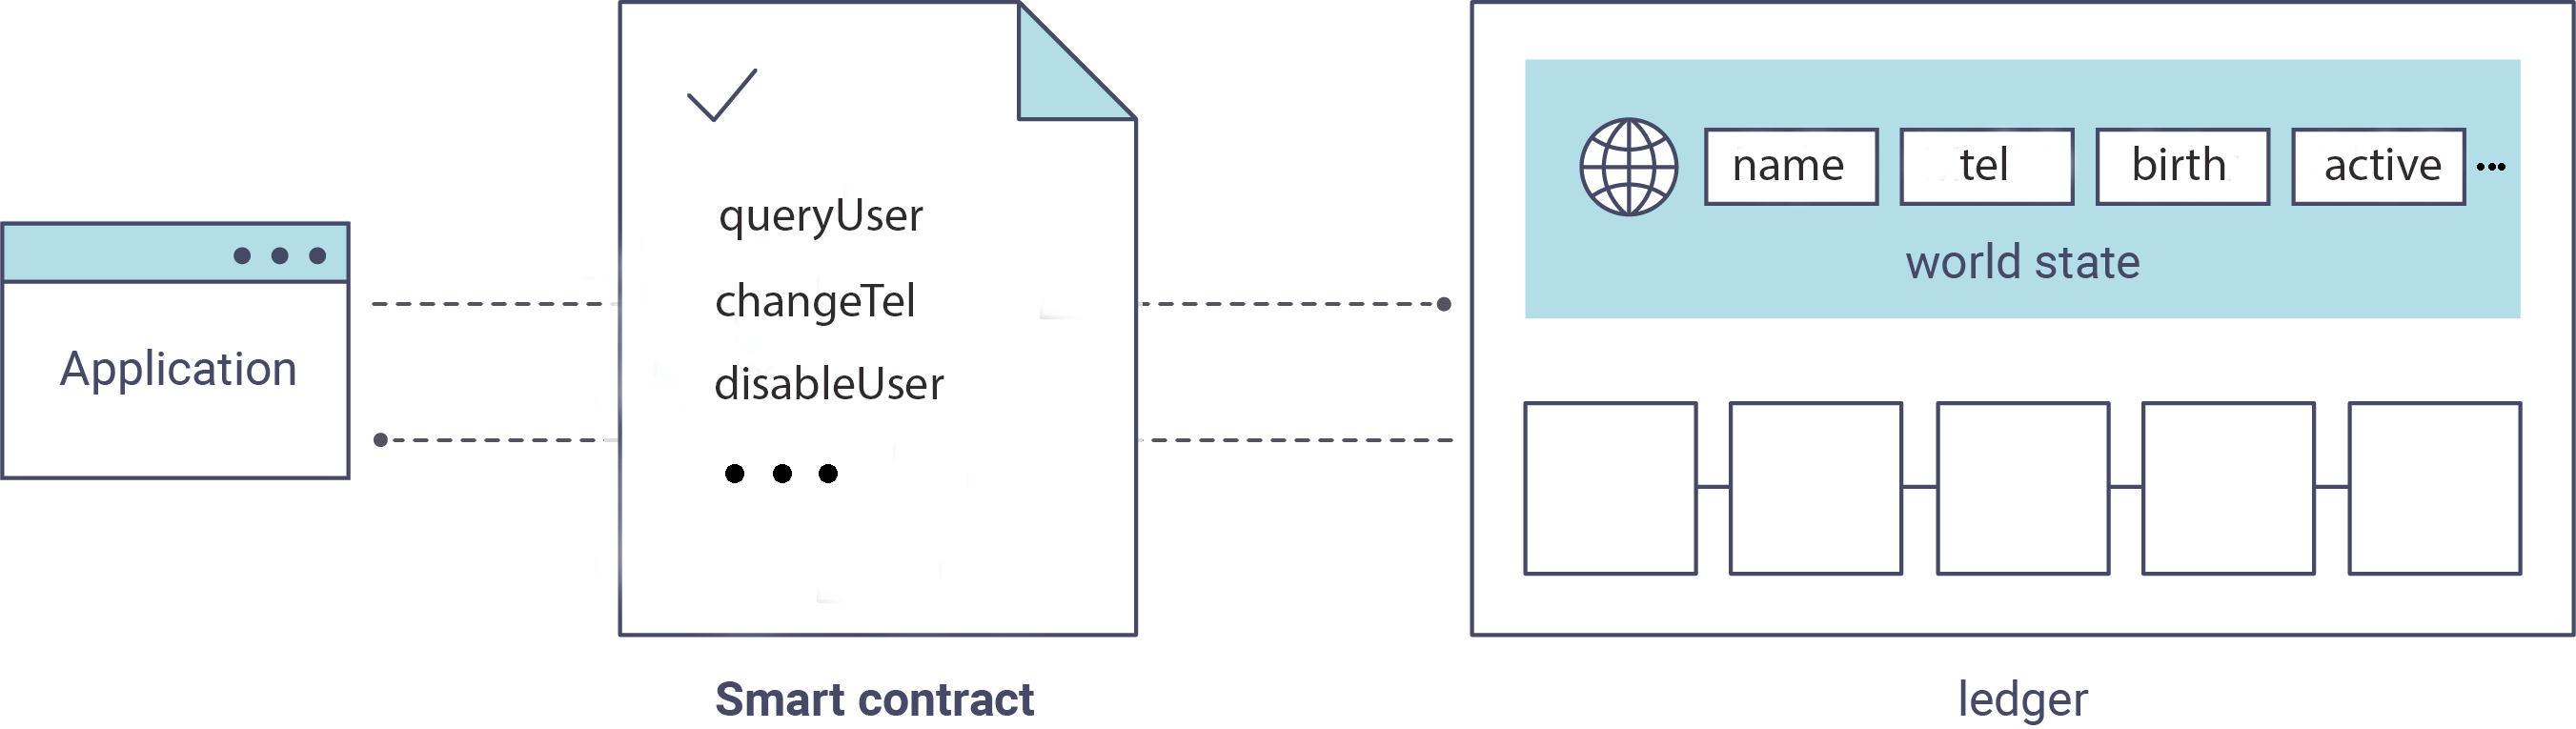
\includegraphics[width=0.9\linewidth]{imgs/smartContractOverview.png}
  \caption{\label{fig:smartContractOverview}Smart Contract Operations Example
  (Original:
  \href{http://hyperledger-fabric.readthedocs.io/en/latest/write_first_app.html}{HLF
  Fabric Documentation})} 
\end{figure}

The network was brought up using the technologies mentioned in the previous
Section and an administrator was enrolled into the network. This step is
required because every action must be verified through a chain of trust and the
administrator is the root CA in the network.

The next step was registering the patient and the doctor. Both the patient and
the doctor invoked the register function of the application and were asked for
a password. After successful register they were presented their assigned
patient number in the format described previously.The password required by the
register function was also stored in the certification store, as well as the
patient number assigned to them. At this point they became active participants
in the network. In this case, the assets that represent their identity were not
created, because they had been exceptionally created before hand by the
administrator to simplify the process. The normal flow would be the creation of
both assets on registration.

\subsection{Data Confidentiality in Fabric}

During the implementation of the system it became clear that additional
measures to secure data was needed. Even tough Fabric is focused towards
privacy and confidentiality, data inserted in a channel between a patient and a
doctor, for example, would be stored in plain text by default. This means that
inside the channel any entity would be able to access all data and see its
contents if the required key to query a specific piece of data was obtained.
To make information confidential some form of obfuscation or encryption could
be used. 

Fabric also features Attribute Based Access Control meaning that the chaincode
logic could be altered to check if some attribute was present on the doctor's
certificate that indicated that he had access to certain patients information.
This could work for application users if there was no other way to access a
network, however if users used a tool like Hyperledger Explorer they could see
the data since the data is stored as plain text, as discussed in the previous
paragraph.

After considering the different possibilities and making some tests it was
decided to use data encryption. The flow of the operations is designed to be
simple. When the patient's data is registered he receives a notification to
keep note of a data key which is used to encrypt data using a traditional
\href{https://en.wikipedia.org/wiki/SHA-2}{SHA-256 encryption algorithm}. The
data was encrypted using
\href{https://www.ibm.com/support/knowledgecenter/en/SSB23S_1.1.0.14/gtps7/s7symm.html}{symmetric
key encryption} with the generated key being stored on the
\href{https://en.wikipedia.org/wiki/X.509}{X.509 certificate} of the respective
client securely. If a patient wanted to share his information with someone he
would give the other entity his data key and that would allow him to decrypt
the encrypted patient's data. To complete this system the key would need to be
set to expire after a set amount of time and refresh itself, as discussed in
Section \ref{futureWork}. The key could always be accessible to the patient by
accessing the data store where Fabric security mechanisms would ensure the
certificate attributes are only accessible to the rightful owner.

With this system in place, the last requirement was fulfilled, and the system
is now considered to be complete regarding the goals of this dissertation.
